\documentclass[tikz,border=2pt]{standalone}
\usepackage{amsmath,amssymb}
\usepackage{pgfplots}
\pgfplotsset{compat=1.18}

\begin{document}
% Covariance as an average product of deviations: points up-right and down-left of the means
% contribute positive products, the other two quadrants negative ones.
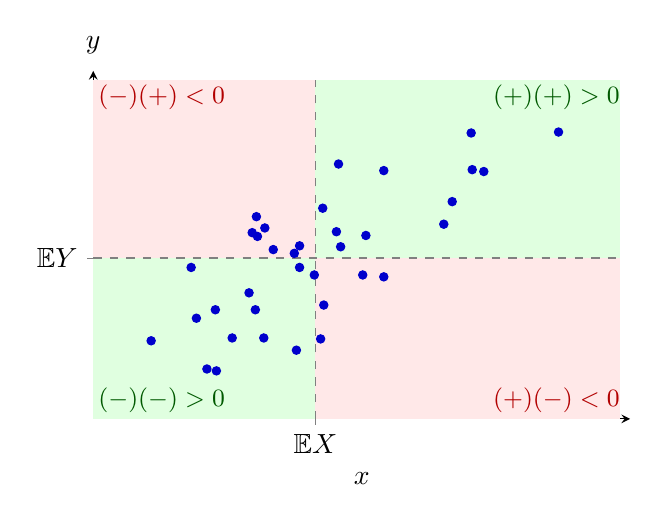
\begin{tikzpicture}
	\begin{axis}[
		axis lines=left, xmin=0.8, xmax=5.9, ymin=0.3, ymax=4.0,
		xtick={2.91}, xticklabels={$\mathbb{E}X$}, ytick={2.01}, yticklabels={$\mathbb{E}Y$},
		xlabel={$x$}, ylabel={$y$}, ylabel style={rotate=-90, anchor=south, at={(axis description cs:0,1.02)}},
		width=8.4cm, height=6cm, clip=false
		]
		\fill[green!12] (axis cs:2.91,2.01) rectangle (axis cs:5.8,3.9);
		\fill[green!12] (axis cs:0.8,0.3) rectangle (axis cs:2.91,2.01);
		\fill[red!9] (axis cs:0.8,2.01) rectangle (axis cs:2.91,3.9);
		\fill[red!9] (axis cs:2.91,0.3) rectangle (axis cs:5.8,2.01);
		\draw[gray, dashed] (axis cs:2.91,0.3) -- (axis cs:2.91,3.9);
		\draw[gray, dashed] (axis cs:0.8,2.01) -- (axis cs:5.8,2.01);
		\addplot[only marks, mark=*, mark size=1.5pt, blue!80!black] coordinates {(5.22,3.35) (2.71,2.06) (1.78,1.37) (2.12,1.16) (4.40,2.95) (1.73,1.91) (1.88,0.83) (3.56,1.81) (2.42,1.16) (2.28,1.64) (2.51,2.10) (2.98,2.54) (2.90,1.83) (2.76,1.91) (3.56,2.94) (2.31,2.28) (3.36,1.83) (3.11,2.29) (2.43,2.33) (4.21,2.61) (2.76,2.14) (4.39,3.34) (3.39,2.25) (2.99,1.51) (2.35,2.45) (4.51,2.93) (3.13,3.01) (2.73,1.03) (1.97,0.81) (2.96,1.15) (1.35,1.13) (4.13,2.37) (2.34,1.46) (3.15,2.13) (2.36,2.24) (1.96,1.46)};
		\node[green!35!black, font=\small] at (axis cs:5.2,3.72) {$(+)(+)>0$};
		\node[green!35!black, font=\small] at (axis cs:1.45,0.5) {$(-)(-)>0$};
		\node[red!70!black, font=\small] at (axis cs:1.45,3.72) {$(-)(+)<0$};
		\node[red!70!black, font=\small] at (axis cs:5.2,0.5) {$(+)(-)<0$};
	\end{axis}
	
\end{tikzpicture}
\end{document}
